\documentclass{newseye_del}

\usepackage[utf8]{inputenc}
\usepackage[backend=biber, sorting=none]{biblatex}
\usepackage{csquotes}
\usepackage[english]{babel}

% Useful package bundled along with this class
% to add person-specific comments (using todonotes)
\usepackage{comments}
% Define author names
\newauthor[Mgw]{Mark}{red}


\addbibresource{references.bib}



%+++++++++++++++++++++++++++++++++++++++++++++
%%%% All details should be filled in here %%%%
% Deliverable number:
\dnum{n.n}
% Deliverable full title
% (as in the description of the action -
% if needed, you may use a subtitle for better printing on the title page)
\title{Full name/title of deliverable (without deliverable number)}
\subtit{}
% Deliverable short title
\shorttitle{Deliverable Short Name (max. 50 chars)}
% Document identifier -
% please refer to the instructions of the quality management deliverable,
% annex A at https://drive.google.com/open?id=1Kgrj2NhfV8CiUIvwVncivTOVAyXn-oWK
% format = NewsEye-Tmm-Dnn-DeliverableShortName-status-vn.n.Extension
\docid{NewsEye-Tmm-Dnn-DeliverableShortName-status-vn.n}
% Lead partner
\resp{XXX}
% Report version
% please refer to the instructions of the quality management deliverable, annex A
\version{1.0}
% Date of completion of this version
\newdate{versiondate}{01}{01}{1900}
% Due date of deliverable
\newdate{duedate}{01}{01}{1900}
% Project month in which the deliverable is due
\duemonth{0}
% Dissemination level: PU, PP, RE or CO (see title page)
\distribution{CO}
% Deliverable type
\type{Report}
% Deliverable status, exactly one these options: Draft, Final or Submitted
\stat{Draft}
% Author and co-authors, please put affiliation in parentheses for all
\mainauthor{Firstname Lastname (XXX)}
\coauthor{First2 Last2 (YYY), First3 Last3 (YYY), \dots}
% Reviewers
\intrew{First1 Last1 (ZZZ), First2 Last2 (ZZZ)}
%+++++++++++++++++++++++++++++++++++++++++++++



\begin{document}

\titlepage

The NewsEye Consortium partner responsible for this deliverable has
addressed all comments received, making changes as necessary.
Changes to this document are detailed in the change log table below.

\textbf{Change Log}\\[5pt]
\begin{tabular}{ |p{2.1cm}|p{1.2cm}|p{3.8cm}|p{7.06cm}|  }
 \hline
 \rowcolor{lightgray} Date & Version & Editor & Summary of changes made\\
 \hline
 03/01/1900 & 1.0 & \makecell{Firstname Lastname \\ (XXX)} & First full draft\\
 \hline
 24/01/1900 & 1.1 & \makecell{Firstname Lastname \\ (XXX)} & Modifications taking reviewer comments into accounts: done this, done that, added this and removed that.\\
 \hline
 27/01/1900 & 2.0 & \makecell{WP leader \\ (YYY)} & Clarifications, typographical errors and adjustments\\
 \hline
 31/01/1900 & 3.0 & \makecell{Coordinator \\ (ZZZ)} & Minor modifications towards submission\\
 \hline
\end{tabular}



\newpage
\section*{Executive summary}
\addcontentsline{toc}{section}{Executive Summary}

The executive summary of a report deliverable is expected to be an
abstract version of it. It should give a quick glimpse of the main
results of the deliverable. In principle, the executive summary
should consist of about 10 to 20 lines of text.

\tableofcontents
\newpage


\section{Section top level}

Text \dots

\subsection{Section 2nd level}
\label{sec:example subsection}

Text \dots

\subsubsection{Section 3rd level}

Text \dots

\section{Report titles}

Deliverables have a title that is defined in the DoA (Description of the  action
-- part A of annex 1 of the grant agreement). This title is referred  to as the
full title of the deliverable. Please stick to the official spelling. It is
important to also define a short title (max 60 characters) for each deliverable
as it can be cumbersome to always use a lengthy (full) title.

\section{File naming}

The project will generate many documents (deliverable reports) and versions of
these reports. It is therefore beneficial to consistently use an agreed file
naming format.

NewsEye-Tmm-Dnn-DeliverableShortName-status-vn.n.Extension

Notice the hyphen between the various elements of the file name.

\begin{itemize}
    \item \textbf{NewsEye:} Each NewsEye report should be preceded by the
      project acronym. Notice, there is only a single spelling of the acronym:
      `NewsEye.
    \item \textbf{Tmm:} Indicating the task number, e.g., `T21' for `Task 2.1'
      following the numbering of the DoA (part A of annex 1 of the grant
      agreement). Notice, there is no dot between the two parts of the task number.
    \item \textbf{Dnn:} Indicating the deliverable identifier, e.g., `D34' for
      `D3.4' following the numbering of the DoA.
      Notice, there is no dot between the two parts of the deliverable number.
    \item \textbf{DeliverableShortName:} This should be based on the formal
      short title of deliverables but `contracted' into a single (no spaces)
      character string using Java class naming convention, e.g., `ExploitationPlan',
      or `MWPrototypeForLibX' or `ProjectWebSite'.
      Avoid underscore, space and other unusual characters.
    \item \textbf{Status:}
      \begin{itemize}
          \item draft = draft version -- indicates that the drafting of the
            report is in progress; The `final draft' is the version sent to reviewers (v1.x);
          \item final = final version as checked and updated by the
            reviewers/WP leader/quality manager.
            It can still evolve before its last version (v2.x) is sent to the
            project administrator;
          \item submitted = submitted version as submitted to the EC by the
            project coordinator (normally v3.0).
      \end{itemize}
    \item \textbf{vn.n:} The version of the report starting from v1.0.
      Once more, conventionally:
      \begin{itemize}
          \item 1.x stands for the draft versions;
          \item 2.x stands for final versions;
          \item 3.x stands for the submitted version (in theory, only 3.0 will exist);
          \item x is an integer, starting with 0, and incremented by 1 for
            each new subversion within the status (`draft', `final', or in rare
            cases `submitted').\footnote{%
              Please note: when using a collaborative platform for co-writing,
              the x number (in 1.x for instance) will remain unchanged.}
      \end{itemize}
    \item \textbf{Extension:} File extension, e.g., `doc' for Microsoft Word
      and `pdf' for Portable Document Format. All deliverables will be
      submitted in PDF format.
\end{itemize}

Examples:
\begin{itemize}
    \item NewsEye-T13-D111-DataGeneration-draft-v1.2.doc
    \item NewsEye-T41-D42-AnalysisOfDataInAGivenContext-final-v2.0.pdf
    \item NewsEye-T83-D82-QualityAssurancePlan-submitted-v.3.0.pdf
\end{itemize}

\section{Change log}

The change log is there to keep track of the changes made to the document.
Whenever changes are made to the document, a new version should be created and
the changes should be briefly summarized in the change log. There is a minimum
of three phases of change log entries. (1) The Deliverable Manager (researcher
responsible for this deliverable) enters changes as he or she develops the
document. (2) The two reviewers and the Quality Manager register the changes
made in the quality assurance phase. Once the Deliverable Manager passes the
report on to the Project Manager, the status should be changed from `draft'
to `final'. (3) The Project Manager registers the changes before submitting
the document. Before he submits the report to the EC, the status should be
changed from `final' to `submitted'.

\section{Document formatting}
\section{Basic formatting}
Use standard \LaTeX formatting to write your document.

Format lists using \verb.\begin{itemize}..
\begin{itemize}
    \item Point 1
		\item Another point
\end{itemize}

Separate paragraphs using blank lines.

If you need to force a page break, use \verb.\newpage..

You can use footnotes using the \verb.\footnote{}. command\footnote{%
	Like this!
}.


\subsection{Headings}

Like in many journals and books, it is a good practice not to use more than 3
levels of headings. If you really need more, then by all means do so, but you
may first consider how to structure the document with a maximum of three heading
levels.

Use the following capitalization style for all headings:

`Text text text text'

Only first term is capitalized (unless, of course, English grammar
capitalization require otherwise) and do not use a full stop at the end.

Notice, there is an empty line before each new heading!

\paragraph{A paragraph title.}
You can also use \verb.\paragraph{}. for small divisions.


\subsection{Paragraph}

The paragraphs are separated by an empty line (not by ad hoc spacing). Each
plain paragraph has the style Normal, which has the following main formatting
features:

\begin{itemize}
    \item Style: Arial
    \item Font size: 10 pt
    \item Alignment: Justified
    \item Spacing: 1.2 lines
\end{itemize}

\subsection{Page set-up}

Format: A4 \\
Left and right margins: 2.54 cm \\
Top and bottom margins: 2.00 cm \\

\subsection{Captions and citations}

Use the following for captions and cross-referencing:

\begin{itemize}
    \item `Table 1' for tables, not `table 1' or `Tab. 1', etc.
    \item `Figure 1' for figures, not `figure 1' or `Fig. 1', etc.
    \item `Section 1.1.1' to cross-reference other sections, not `section 1.1.1'
      or `S. 1.1.1', etc.
\end{itemize}


Do not abbreviate the word `Equation' to `eq', `Eqn', etc.

Table captions should be placed \textbf{above} the table and figure captions
\textbf{below} the figure. The captions should succinctly describe the content
of the table or figure.


\subsection{Tables}

\subsection{Figures}

Good figures/diagrams are even more difficult to produce than tables. Figures
should contain legends explaining the symbols in the figure. Avoid surrounding
of the figure with a box outline. If there are different parts to a figure (e.g,
(a), (b), (c)), indicate these clearly. Make sure that the labels within a
figure/diagram are spelled consistently within the figure/diagram and are also
consistently spelled in the text. Make sure that caption appears on the same
page as the figure. The figure caption is below the figure! See an example of a
figure and its caption below (\textit{not currently reproduced in Latex}).

The figure caption should follow the sentence style layout and end with a full
stop. The figure caption as well as the figure should be left-aligned.

To include figures inline, using \verb.\begin{figure}[H]..
For example, the following chart provides an overview on the main components of the project:

\begin{figure}[H]
	\centering
	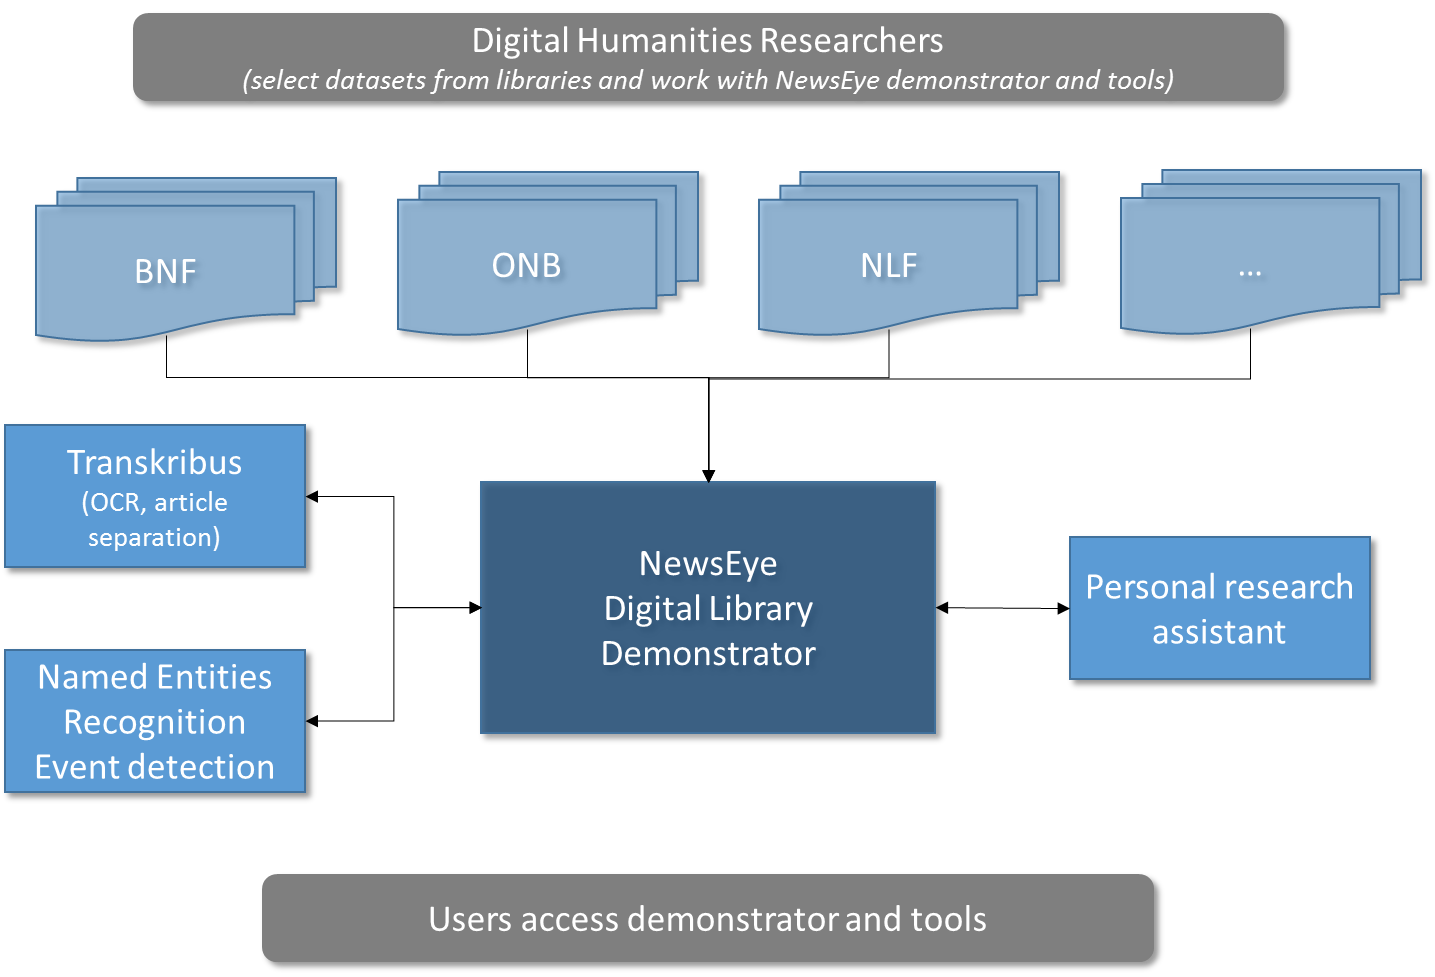
\includegraphics[width=0.7\textwidth]{overviewNewsEye.png}

	\caption{Overview of NewsEye}
	\label{fig:place}
\end{figure}


\subsection{Footnotes}

This\footnote{Usually the footnote is at the bottom of the same page where the
footnote is cited and the font size is only 9 pt. Footnotes are useful to for
including nasty-looking long Web references which would look terrible if used in
the main flow of the text.} is a footnote.


\section{Language and notation} There are a few things one should consider when
writing documents in terms of language. The question is not deeply philosophical
in the sense of whether one or the other approach is fundamentally correct (or
wrong). It is more a case of maintaining a certain level of consistency across
the project.

Since \textbf{British/UK English} is the official version of English within the
EC, we should adopt this, rather than using different forms of English ranging
from US to Australian to Caribbean through to Zimbabwean. So (a) use a
spell-checker, and (b) set it to UK English!

\textbf{Quotation marks.} UK English (unlike US), use single quotation marks
(`X') instead of double quotation marks (``X''). At least maintain consistency
within a document.

\begin{itemize}
    \item It is claimed that Y is `superior' to X.
    \item `Good morning, Dave,' greeted HAL.
\end{itemize}

Do not use quotation marks to indicate emphasis -- use italics, bold or
underline style instead.

Avoid \textbf{colloquial English} and highly informal expressions in scientific
writing. The Web is full of good guidelines on writing scientific documents and
the use of English.

The accepted standard for separating \textbf{orders of magnitude} in large
figures is not `,' or `'' (quotation mark) or `.', but a non-breaking (small)
space.

\begin{itemize}
    \item This is bad: 1,000,000 or 1.000.000 or 1'000'000 (very bad!)
    \item This is good: 1~000~000. For four-digit numbers, no separation
      symbol is usually used, e.g., 1000, 9300.
\end{itemize}

\textbf{Capitalization.} Use capitalization according to English grammar rules,
not according to what you read in papers, especially in IT papers, as IT people
(and some other engineering folks) are notoriously poor in adhering to good
standards of English grammar and expression. Apart from few exceptions, you
capitalize words that are either a name or a kind of title, and, obviously, at
the beginning of a sentence. So capitalizing terms like `machine learning',
`data mining', etc. is grammatically incorrect (unless they occur in a name or
title). Avoid capitalization of the word `grid' and similar words, unless
grammar rules suggest otherwise. Also, you do not capitalize a term just because
the acronym comes in capital letters, so it is `case-based reasoning (CBR)' and
not `Case-Based Reasoning (CBR)'. Incidentally, the whole point of introducing
abbreviations like `Web services (WS)' in a text is that the abbreviation,
instead of the full version, is to be used subsequently. Hence, it does not make
sense, as it is sometimes seen, to introduce the same abbreviation more than
once. Sometimes, if too many abbreviations are introduced and used, the text
becomes unreadable, so use this mechanism only for the most important concepts
and use the full terms for most other notions.

Capitalization rules:\\
\url{http://andromeda.rutgers.edu/~jlynch/Writing/c.html}\\
\url{http://www.grammarbook.com/punctuation/capital.asp}

\textbf{Tense.} Use \textbf{past tense} when describing activities and tasks
(experiments, developments, etc.) carried out in the past.

\begin{itemize}
    \item A test bed \textbf{was} set up to \dots
    \item The evaluation \textbf{revealed} that \dots
\end{itemize}

Use \textbf{present tense} when describing the ideas, design, systems, etc. that
exist in the present.

\begin{itemize}
    \item The system supports the following exchange formats \dots
    \item A key property of the system is its ability to \dots
\end{itemize}


\textbf{Large numbers.} Use explicit format or scientific notation for large
numbers

Use 1~200~000~000, not 1.2bn or 1,200,000,000\\
Or use $1.20\cdot10^9$ or  $1.20\times10^9$

\textbf{Small numbers.} As usual, unless in tables and similar things, use {one,
two, \dots, twelve} for numbers < 13, and \{13, 14, \dots\} for large numbers.

\textbf{Numbers and units.} Use small space (In Latex: \textbackslash, or
\textasciitilde) to separate figures from units. E.g.,

\begin{itemize}
    \item 10~GB, not 10GB
    \item 2.13~s, not 2.13s
\end{itemize}

\textbf{Bits, bytes and pieces.} Use the following terms and abbreviations for
bytes. By the way, sometimes it is better to use the full term than the
abbreviation.

Bits:\\
\begin{tabular}{lll}
    kb or Kb & kilobit & $10^3$ \\
    Mb & megabit & $10^6$ \\
    Gb & gigabit & $10^9$ \\
    Tb & terabit & $10^{12}$ \\
    Pb & petabit & $10^{15}$ \\
    Eb & exabit & $10^{18}$ \\
    Zb & zettabit & $10^{21}$ \\
    Yb & yottabit & $10^{24}$ \\
\end{tabular}

Bytes:\\
\begin{tabular}{lll}
    kB or KB & kilobyte & $10^3$ \\
    MB & megabyte & $10^6$ \\
    GB & gigabyte & $10^9$ \\
    TB & terabyte & $10^{12}$ \\
    PB & petabyte & $10^{15}$ \\
    EB & exabyte & $10^{18}$ \\
    ZB & zettabyte & $10^{21}$ \\
    YB & yottabyte & $10^{24}$ \\
\end{tabular}

\textbf{Precision, accuracy and significance.} In the decimal system, the
\textbf{accuracy} of a number $x$ is given by the number of \textbf{significant}
decimal digits to the right of the decimal point in $x$, the \textbf{precision}
of $x$ is the total number of significant decimal digits.
\url{http://mathworld.wolfram.com/Precision.html}

When a number is expressed in scientific notation, the number of
\textbf{significant} digits (or significant figures) is the number of digits
needed to express the number to within the uncertainty of calculation. For
example, if a quantity is known to be $1.234 ~ \pm ~ 0.002$, four figures would
be significant. \url{http://mathworld.wolfram.com/SignificantDigits.html}

Unless there is a good reason, \textbf{do not} use more than three fractional
digits or places (the number of digits following the point). For example, you
may have `measured' the run time of a grid data mining process as 12.346789~s
(probably difficult if not impossible -- but system clocks spit out all sorts of
things), you need to think if it is really of importance to report all those
fractional digits, maybe 12.35~s will do.

\textbf{Other issues.} Avoid overly long sentences. Certain studies suggest that
sentence over approximately 20 words become difficult to understand and should
therefore be avoided. An example of a long sentence is shown below.

Now if nature should intermit her course and leave altogether, though it were
but for awhile, the observation of her own laws; if those principal and mother
elements of the world, whereof all things in this lower world are made, should
lose the qualities which now they have; if the frame of that heavenly arch
erected over our heads should loosen and dissolve itself; if celestial spheres
should forget their wonted motions, and by irregular volubility turn themselves
any way as it might happen; if the prince of the lights of heaven which now as a
giant doth run his unwearied course, should, as it were through a languishing
faintness, begin to stand and to rest himself; if the moon should wander from
her beaten way, the times and seasons of the year blend themselves by disordered
and confused mixture, the winds breathe out their last gasp, the clouds yield no
rain, the earth be defeated of heavenly influence, the fruits of the earth pine
away as children at the withered breasts of their mother no longer able to yield
them relief --- what would become of man himself, whom these things now do all
serve?

Incidentally, the opposite, too many short sentences, may also undermine the
scientific character of a technical/scientific document. For example:

BlindEye is the user interface. It has many options. For example, the `save'
option. Its function is to save user files. The file size is limited to 10~MB.
Typically, this is not a problem. But biologists may require large files. This
study addresses this issue. \dots

\textbf{Other.} There are a number of other things one should consider when
writing technical and scientific reports. There is a lot of material on the Web
on this.

\section{Source code etc.}
You can use the \texttt{minted} package for formatting source code.


\section{References}
There are infinite options of how to format references and their citations
within a document. Since there are many different partners and possible
preferences from different domains, the best solution is not to define this
globally. However, one should make sure that within a single document the
notation for references and their citations should be consistent.

You can cite papers by adding them to \texttt{references.bib}
and then including the \verb.\cite{}. command to refere to them:
\cite{Crane2017}.

To update your bibliography, you need to run \texttt{pdflatex main},
then \texttt{biber main}, then \texttt{pdflatex main} again.


\href{https://www.newseye.eu/}{URLs} should be included using the \verb.\href{}{}. command.

Refer to sections within the document by placing a \verb.\label{myname}.
command at the start of the section, then using the \verb.\ref{myname}.
command to refer to it, as in the case of the
section~\ref{sec:example subsection}. Use the same method for referring
to figures, like fig.~\ref{fig:place}.


% Shows all the todos in the document
% Remove this before submission!
%\listoftodos{}



% Show the bibliography at the end
\newpage
\printbibliography

\end{document}
